\begin{figure}[h!]
    \begin{center}
    \caption{Effects on Access to Health Services}\label{fig:13}
    \begin{subfigure}{0.48\textwidth}
        \caption{\scriptsize Prenatal Visits Ignored}\label{fig:13a}
        \centering
        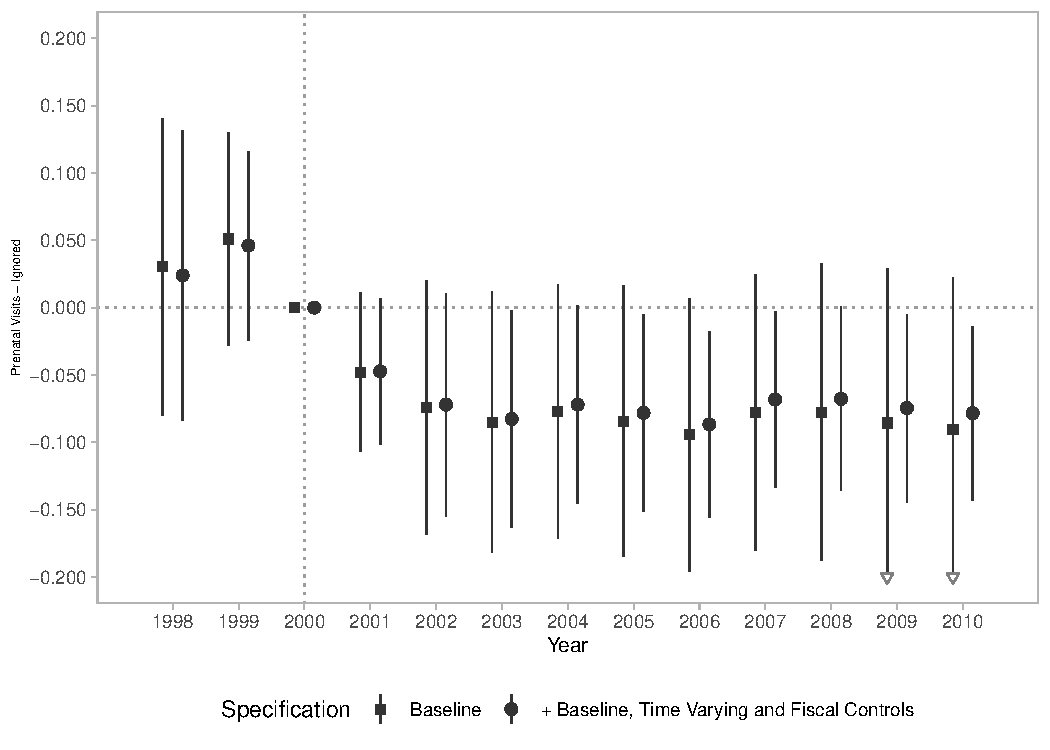
\includegraphics[width=\textwidth]{plots/birth_prenat_ig_dist_ec29_baseline_dist_ec29_baseline_13.pdf}
    \end{subfigure}
    \begin{subfigure}{0.48\textwidth}
        \caption{\scriptsize Prenatal Visits None}\label{fig:13b}
        \centering
        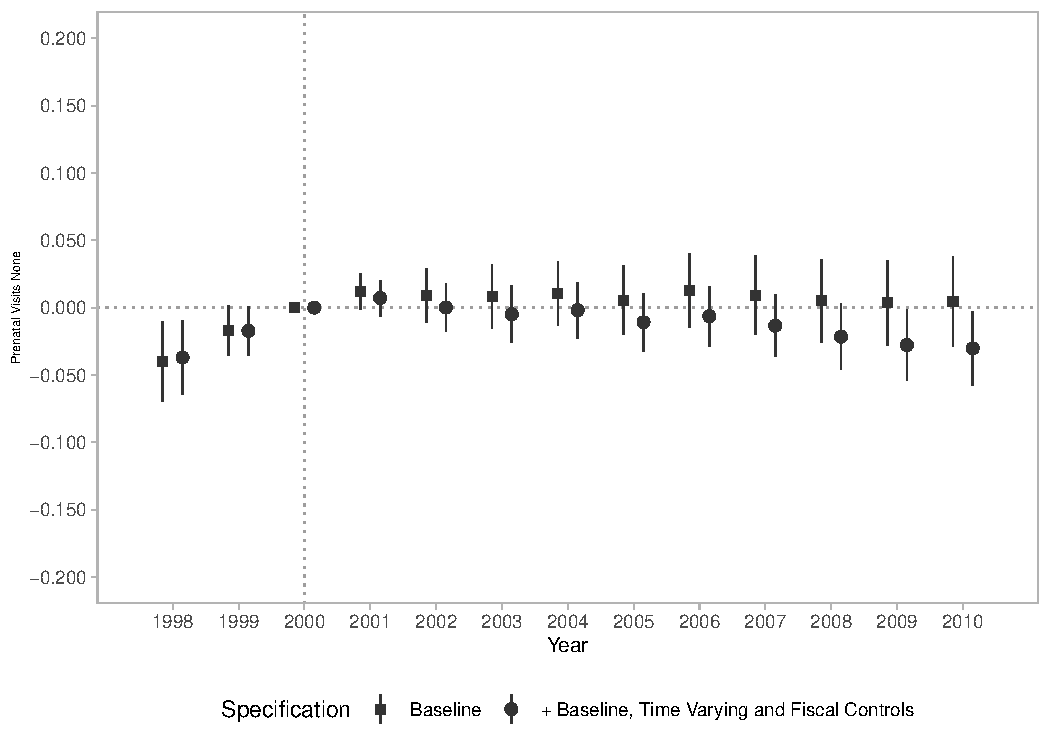
\includegraphics[width=\textwidth]{plots/birth_prenat_0_dist_ec29_baseline_dist_ec29_baseline_13.pdf}
    \end{subfigure}
    \begin{subfigure}{0.48\textwidth}
        \centering
        \caption{\scriptsize Prenatal Visits 1-6}\label{fig:13c}
        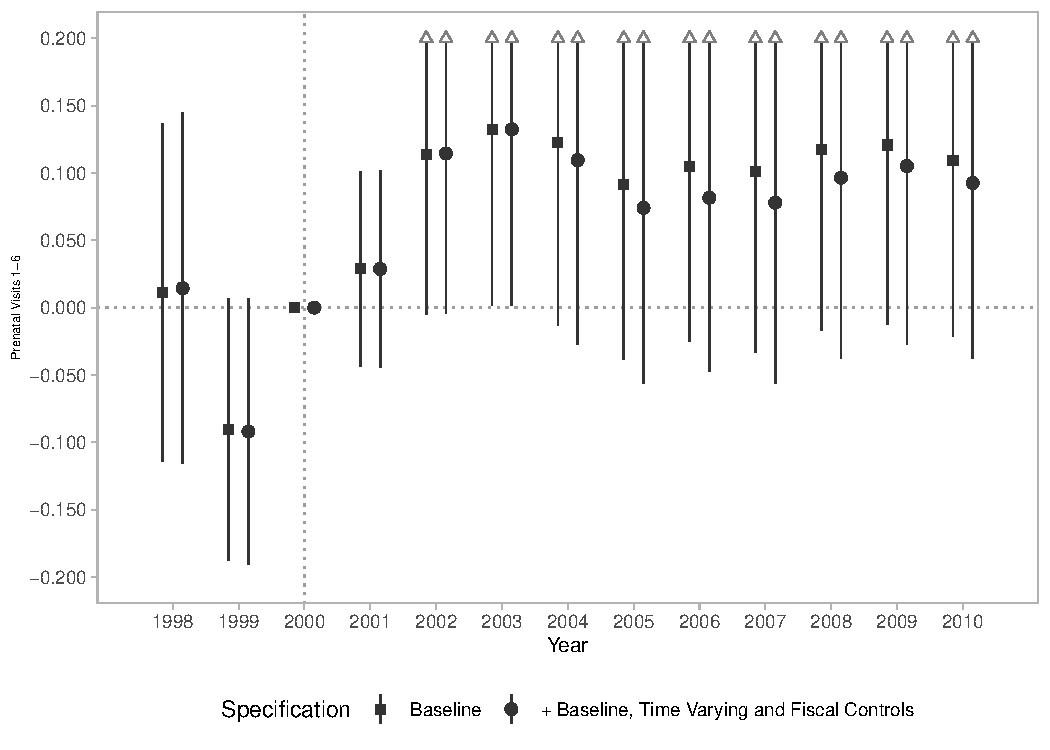
\includegraphics[width=\textwidth]{plots/birth_prenat_1_6_dist_ec29_baseline_dist_ec29_baseline_13.pdf}
    \end{subfigure}
    \begin{subfigure}{0.48\textwidth}
        \centering
        \caption{\scriptsize Prenatal Visits 7+}\label{fig:13d}
        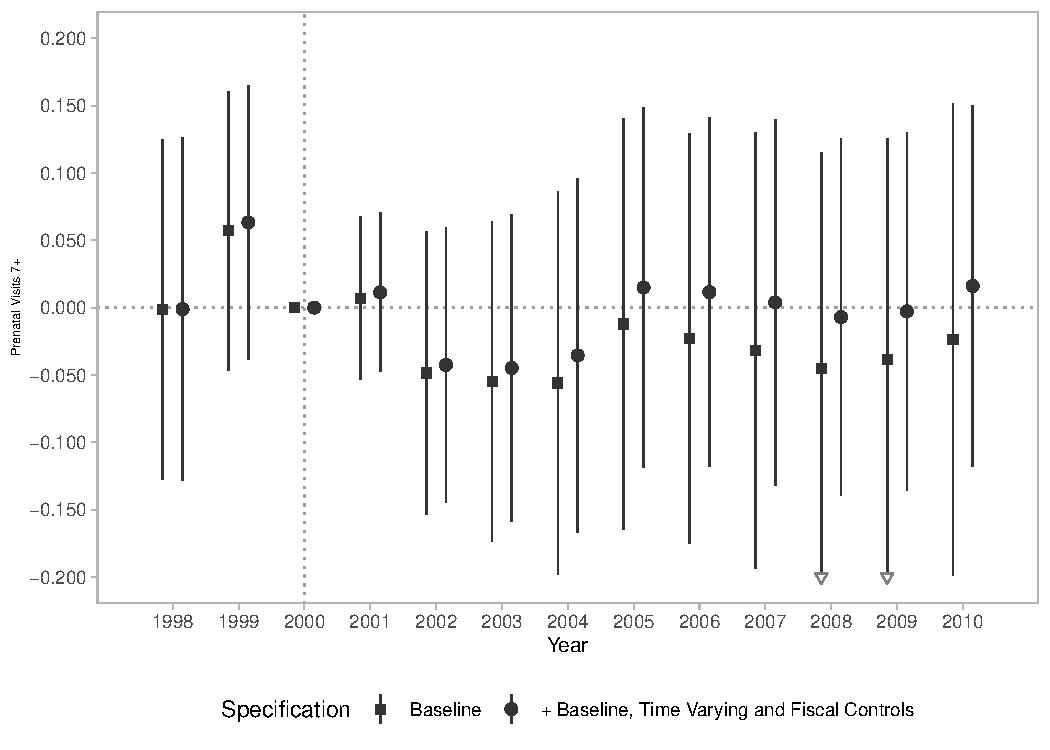
\includegraphics[width=\textwidth]{plots/birth_prenat_7_plus_dist_ec29_baseline_dist_ec29_baseline_13.pdf}
    \end{subfigure}
        
    
    \end{center}
    
    \scriptsize{Notes: The number of observations is 64481. DiD Estimates from Equation \ref{eq:2}. Independent variable is the distance to the EC/29 target in p.p. Square dots represent the baseline model with municipality and state-year fixed effects. Round dots represent fully saturated specification (Column 4 in regression Tables). Lines represent 95\% confidence intervals. Arrows, when present, indicate confidence intervals out of the plot bounds. Standard errors are clustered in the municipality level.}

    
\end{figure}